\subsubsection*{Misura non ripetibile di lunghezza}
$

$
  \begin{figure}[H]
$
  \centering
$
   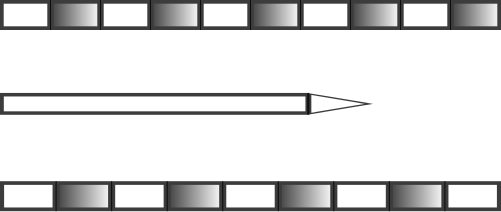
\includegraphics[width=\textwidth]{../immagini/mozzicone.png}
$
   \label{figure:nonio}
$
   \caption{il nonio decimale}
$
  \end{figure}
$

$
In figura \ref{figure:nonio} osserviamo un mozzicone di matita tra due regoli graduati, che
$
vogliamo utilizzare come strumenti per una misura didattica della lunghezza del mozzicone.
$
\newline
$

$
Prima di tutto, osserviamo i due strumenti di misura. Si tratta di due righelli graduati con un passo
$
diverso. Infatti, pur avendo la stessa lunghezza totale, contano uno nove unità e il secondo dieci. Il primo righello,
$
di conseguenza, possiede una {\bf sensibilità} {\bf u} leggermente inferiore alla sensibilità {\bf v} del secondo.
$

$
Possiamo determinare una prima misura della lunghezza della matita in uno di questi due modi:
$

$
\begin{center}
$
  \begin{math}
$
    8~v~<~L~<~9~u~~~~oppure~~~~L~=~8.5~\pm ~0,5~u
$
  \end{math}
$
\end{center}
$
\begin{center}
$
  \begin{math}
$
    7~u~<~L~<~8~v~~~~oppure~~~~L~=~7.5~\pm ~0,5~v
$
  \end{math}
$
\end{center}
$

$
La prima misura è affetta da un errore relativo $\Delta L~=~\frac{v}{L}~=~frac{1}/{8}=0.13~=~13\%$, e la seconda da un
$
errore relativo $\Delta L~=~\frac{v}{L}~=~frac{1}/{7}=0.14~=~14\%$. Oggettivamente non è granché, ma non possiamo far
$
meglio per questi motivi:
$
\begin {itemize}
$
\item I regoli sono graduati con un passo grossolano e quindi sono poco sensibili.
$
\newline
$
Probabilmente, il vostro occhio (che
$
è più sensibile delle barre graduate) è in grado di proporre una stima migliore, ma per riuscirci siete costretti a
$
cercare dei riferimenti (cioè degli strumenti di misura) aggiuntivi. Noi dobbiamo riflettere
$
esclusivamente sulle proprietà dei righelli.
$
\item Il nostro metodo di misura è piuttosto ingenuo e non sfrutta adeguatamente gli strumenti disponibili.
$
\newline
$
Infatti, entrambi i regoli sono allineati alle estremità di sinistra con
$
la matita, come siamo sempre stati abituati a fare. Questa scelta è molto comoda, perché ci dà
$
certezza che,
$
ripetendo cento volte la misura allo stesso modo, otterremmo cento volte lo stesso risultato. In termini tecnici, si
$
dice che abbiamo scelto di effettuare una misura {\bf non ripetibile}.
$
\end{itemize}
$

$
Vediamo ora come, modificando di poco il {\slshape metodo} di misura, è possibile migliorarne la qualità.
$
\newline
$
Dopo aver riprodotto fedelmente una delle due scale su una striscia di carta, allineate un'estremità della striscia
$
alla punta della matita, come nella figura \ref{figure:nonio2}.
$
Adesso le tacche iniziali della due strisce sono disallineate tra loro, di una quantità uguale allo spazio
$
contrassegnato in figura con {\bf x}. {\bf x} è l'errore della nostra misura. Ma siccome rappresenta una
$
quantità inferiore al passo del regolo, fino ad ora non abbiamo potuto valutarla.
$
\newline
$
Se considerate ora, a due a due, le
$
tacche successive, vi accorgerete che il disallineamento si riduce di molto. Questo accade perché le unità delle due
$
scale sono differenti di un decimo tra loro. In particolare, la scala che abbiamo spostato a fianco della matita
$
utilizza unità più lunghe, quindi tende ad avvicinare le proprie tacche alla striscia precedente di un piccolo passo.
$
Quando osserviamo la sovrapposizione la striscia superiore è rimasta indietro per 6 volte successive, cioè 6 decimi
$
della propria lunghezza. Aggiungendo questi 6 decimi alla distanza distanza incognita si ottiene esattamente una unità.
$
Potremmo rappresentare questa affermazione con l'equazione seguente:
$
\begin{center}
$
\begin{math}
$
x~+6~\frac{u}{10}~=~u
$
\end{math}
$
\end {center}
$
 Quindi, possiamo concludere che il mozzicone oltrepassa di 4 decimi di unità e scriveremo:
$
\begin{center}
$
  \begin{math}
$
    7.35~u~<~L~<~7.45~u~~~~oppure~~~~L~=~7.4~\pm ~0,05~u
$
  \end{math}
$
\end{center}
$

$
  \begin{figure}[H]
$
  \centering
$
   \includegraphics[width=\textwidth]{../immagini/mozzicone2.png}
$
   \label{figure:nonio2}
$
   \caption{il nonio decimale}
$
  \end{figure}
$
Se avete capito:
$
\begin{itemize}
$
\item Calcolate la precisione di questa nuova misura.
$
\item Ripetete la misura spostando la striscia superiore, anzichè
$
quella inferiore e cercate di capire come bisogna adattare il procedimento\footnote{scoprirete che è più comodo.}.
$
\item Esprimete i risultati nelle unità di
$
misura {\bf v} della striscia composta di nove elementi.
$
\end{itemize}
$

$

$
La tecnica illustrata è alla base del funzionamento del nonio\footnote{
$
\url{http://it.wikipedia.org/wiki/Nonio_(strumento_di_misura)}} e del
$
calibro\footnote{\url{http://it.wikipedia.org/wiki/Calibro}}, strumenti che permettono di misurare lunghezze con una
$
risoluzione superiore alle possibilità dell'occhio umano.
$
